\documentclass[letterpaper,11pt]{article}
\usepackage{amsmath}
\usepackage[letterpaper,margin=1in,includehead=true]{geometry}
\usepackage{comment}
\usepackage{graphicx}
\usepackage{fancyhdr}
\pagestyle{fancy}
\usepackage{color}
\usepackage{multicol}

%%%%%%%%%%%%%
\usepackage{pgfplots}
\usetikzlibrary{calc}
\usepackage{wrapfig}
\usepackage{enumitem}

\newcounter{mycounter}
\newenvironment{noindlist}
 {\begin{list}{\arabic{mycounter}.~~}{\usecounter{mycounter} \labelsep=0em \labelwidth=0em \leftmargin=0em \itemindent=0em}}
 {\end{list}}

%To print solutions, use \solutionstrue
%To repress solutions, use \solutionsfalse
%\sol takes two arguments. #1 is the vertical length. #2 is the text.

\newif\ifsolutions
\solutionstrue
\ifsolutions
    \newcommand{\sol}[2]{\begin{minipage}[c][#1]{\linewidth}{\textcolor{blue}{\textbf{Solution:}}\quad \textcolor{blue}{#2}}\end{minipage}}
    \newcommand{\opsol}{1}
\else
    \newcommand{\sol}[2]{\begin{minipage}[c][#1]{\linewidth}{\vfill}\end{minipage}}
    \newcommand{\opsol}{0}
\fi

\newcommand{\unenumerate}[1]{\setcounter{saveenum}{\value{enumi}}\end{enumerate}
	\noindent #1
	\begin{enumerate} \setcounter{enumi}{\value{saveenum}}}

\newcounter{saveenum}

\def\changemargin#1#2{\list{}{\rightmargin#2\leftmargin#1}\item[]}
\let\endchangemargin=\endlist

\begin{document}

\lhead{\bf Math 241: Calculus I}
\rhead{\bf Worksheet Questions}
\tableofcontents

\newpage

\section{Functions and Limits}
\subsection{Math 140 Review}
\begin{enumerate}
  \item If $f(x) = \sqrt{x+5}-\sin\left( \dfrac{\pi}{2}x\right)$, then find the exact value of $f\left(\dfrac{2}{3}\right)$
  \item Find the domain of each function:
  \begin{enumerate}
    \item $f(x) = \sqrt{2-5x}$
    \item $f(x) = \dfrac{1}{x\sqrt{x+3}}$
    \item $f(x) = \sqrt[3]{2-7x}$
  \end{enumerate}
  \item Find the difference quotient of each function:
  \begin{enumerate}
    \item $f(x) = 2x^2+x$
    \item $f(x) = \dfrac{1}{x+1}$
  \end{enumerate}
  \item Decompose the following functions $F(x)$ into three simpler functions $f,g,h$ so that $F(x) = (f\circ g\circ h)(x)$. Do not use the identity/trivial function for $f,g$ or $h$.
  \begin{enumerate}
    \item $F(x) = \sqrt{x^2+4}$
    \item $F(x) = \sin^2(2x+1)$
    \item $F(x) = \tan(\cos(x^3))$
  \end{enumerate}
\end{enumerate}

\newpage
\subsection{The Limit of a Function}
\begin{enumerate}
  \item The graph of $f(x)$ is drawn below. Find the following values and limits if they exist. If the limit is $+\infty$ or $-\infty$ specify which  instead of ``does not exist."
  \begin{center}
    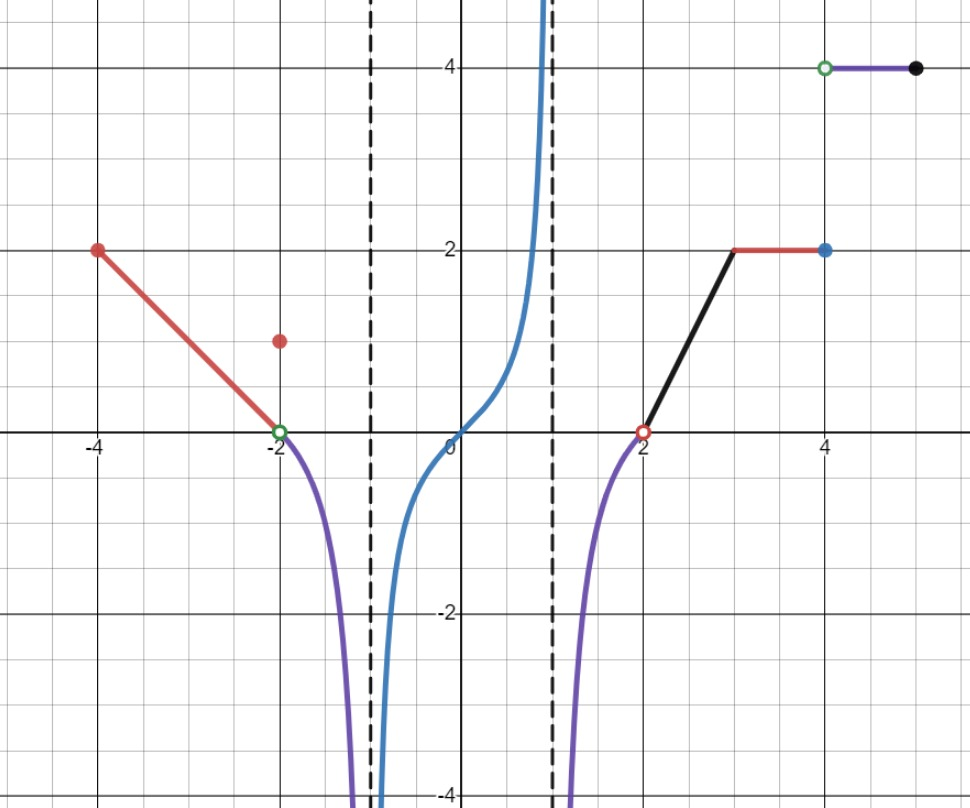
\includegraphics[width=0.75\textwidth]{images/limits1.jpeg}
  \end{center}
  \begin{enumerate}
    \begin{multicols}{2}
      \item $\displaystyle\lim_{x\to -2^-} f(x)$
      \item[]
      \item $\displaystyle\lim_{x\to -2^+} f(x)$
      \item[]
      \item $\displaystyle\lim_{x\to -2} f(x)$
      \item[]
      \item $f(-2)$
      \item[]
      \item $\displaystyle\lim_{x\to -1^-} f(x)$
      \item[]
      \item $\displaystyle\lim_{x\to -1^+} f(x)$
      \item[]
      \item $\displaystyle\lim_{x\to -1} f(x)$
      \item[]
      \item $\displaystyle\lim_{x\to 1^-} f(x)$
      \item[]
      \item $\displaystyle\lim_{x\to 1^+} f(x)$
      \item[]
      \item $\displaystyle\lim_{x\to 2^-} f(x)$
      \item[]
      \item $\displaystyle\lim_{x\to 2^+} f(x)$
      \item[]
      \item $\displaystyle\lim_{x\to 2} f(x)$
      \item[]
      \item $f(2)$
      \item[]
      \item $\displaystyle\lim_{x\to 4^-} f(x)$
      \item[]
      \item $\displaystyle\lim_{x\to 4^+} f(x)$
      \item[]
      \item $f(4)$
      \item[]
    \end{multicols}
  \end{enumerate}
\end{enumerate}

\newpage
\subsection{Calculating Limits using Limit Laws}
\begin{enumerate}
  \item Using the rules for limits, compute the following limits. If the limit is $\pm \infty$ state which. If the limit does not exist, write DNE. \emph{Don't forget to keep the limit notation until you take the limit!}
  \begin{enumerate}
    \item $\displaystyle\lim_{x\to 3} \dfrac{x^2-4x+3}{x^2-9}$
    \item $\displaystyle\lim_{x\to 2} \dfrac{x^2+3x-2}{x-1}.$
    \item $\displaystyle\lim_{x\to 2^+} \dfrac{x^2-2x-8}{x^2-4x+4}$
    \item $\displaystyle\lim_{x\to 0} \dfrac{x^2-x}{x(x+2)}$
  \end{enumerate}
\end{enumerate}

\newpage
\subsection{Precise Definition of a Limit}
\subsection{Continuity}

\section{Derivatives}
\subsection{Derivatives and Rate of Change}
\subsection{Derivative as a Function}
\subsection{Differentiation Formulas}
\subsection{Derivatives of Trigonometric Functions}
\subsection{The Chain Rule}
\subsection{Implicit Differentiation}
\subsection{Rates of Change in Sciences}
\subsection{Related Rates}
\subsection{Linear Approximation and Differentials}

\section{Applications of Derivatives}
\subsection{Maximum and Minimum Values}
\subsection{The Mean Value Theorem}
\subsection{How Derivatives Affect the Shape of a Graph}
\subsection{Limits at Infinity}
\subsection{Summary of Curve Sketching}
\subsection{Graphing with Calculus}
\subsection{Optimization Problems}
\subsection{Newtons Method}
\subsection{Antiderivatives}

\section{Integrals}
\subsection{Areas and Distances}
\subsection{The Definite Integral}
\subsection{The Fundamental Theorem of Calculus}
\subsection{Indefinite Integrals and Net Change Theorem}
\subsection{The Substitution Rule}

\section{Applications of Integration}
\subsection{Areas Between Curves}
\subsection{Volumes}
\subsection{Volumes by Cylindrical Shells}
\subsection{Work}
\subsection{Average Value of a Function}





































\begin{enumerate}
\item  Convert between degrees and radians:

\end{enumerate}
\end{document}
